\documentclass[calculator,datasheet,handbook]{exam}
% The full list of class options are
% calculator : Allows approved calculator use.
% datasheet : Adds a note that data sheet are attached to the exam.
% handbook : Allows the use of the engineering handbook.
% resit : Adds the resit markings to the paper.
% sample : Adds conspicuous SAMPLE markings to the paper
% solutions : Uses the contents of \solution commands (and \solmarks) to generate a solution file

\coursecode{EG3019}%
\coursetitle{Advanced Transport Processes}%
\examtime{9~am -- 12~pm}%
\examdate{27}{01}{2012}%
\examformat{Candidates must attempt \textit{all} questions from {P}{A}{R}{T} {A} \\
  {A}{N}{D} \textit{two} questions from \textit{three} in {P}{A}{R}{T}
  {B}.}

\begin{document}
\part{Answer ALL Questions}
%%%%%%%%%%%%%%%%%%%%%%%%%%%%%%%%%%%%%%%%%%%%%%%%%%%%%%%%%%%%%%%%%%%%%%%%%%%%%%%%
%%%%%%%%%%%%%%%%%%%%%%%%%%%%%%%%%%%%%%%%%%%%%%%%%%%%%%%%%%%%%%%%%%%%%%%%%%%%%%%%
\begin{question}\vspace{-2\baselineskip}
  \begin{enumerate}[a)]
  \item Write down the expressions for the Prandtl number and the
    Grashof number which are used to correlate heat transfer data for
    natural convection from a heated, or cooled, vertical
    surface. Define every term and describe the physical
    interpretation of the dimensionless numbers.%
    \marks{5}\solution{%
      The Prandtl number is defined as
      \begin{align*}
        \text{Pr} = \frac{\mu\,C_p}{k}
      \end{align*}
      where $\mu$ is the fluid viscosity, $C_p$ is the fluid heat
      capacity and $k$ is the thermal conductivity. The Prandtl
      number is a ratio of the momentum to thermal transport in a
      fluid.  \solmarks{2} 

      The Grashof number is the analog of the Reynolds number for
      convective flow and is the ratio of buoyancy and viscous
      forces in the fluid. It is defined as
      \begin{align*}
        \text{Gr}=\frac{g\,\beta \left(T_w - T_\infty\right)\,L^3}{\nu^2}
      \end{align*}
      Where $g$ is the gravitational acceleration, $\beta$ is the
      thermal expansion coefficient, $T_w$ is the wall temperature,
      $T_\infty$ is the bulk temperature, $L$ is the characteristic
      length scale and $\nu$ is the kinematic viscosity.
      \solmarks{3}%
    }
  \item The wall of a furnace was measured to be at a temperature of
    $T_w=60$~${}^\circ$C when the ambient air temperature is at
    $T_\infty=10$~${}^\circ$C. The wall is 3~m high, 5~m wide, and has
    a surface emissivity of $\varepsilon=0.7$. The properties of air
    are given in the table below.
    \begin{center}
      \begin{tabular}{|c|c||c|c|}\hline
        $\mu$ & $1.78\times10^{-5}$~Pa~s & 
        $\rho$ & 1.2~kg/m${}^3$\\\hline
        $k$ & 0.02685~W/m~K & $C_p$ & 1.005~kJ/kg~K\\\hline
      \end{tabular}
    \end{center}
    \begin{enumerate}[i)]
    \item Determine the convective flow regime of the air, noting that
      the critical Grashof number is $\text{Gr}\approx 4\times10^8$.%
      \marks{5}\solution{%
        Here we must calculate the Grashof number. The key
        characteristics are :
        \begin{itemize}
        \item The thermal compressibility $\beta$ is given by
          $\beta=1/T$ for an ideal gas, which is a good approximation
          for atmospheric air.
        \item The properties in the Grashof number should be evaluated at
          the film temperature $T_f = \left(T_w+T_\infty\right)/2$. 
        \item The above rule only applies to the thermal
          compressibility in this question, as the other properties are
          unavailable.
        \item For a vertical plate/wall, the characteristic length is the
          height of the wall.
        \end{itemize}
        \solmarks{3}%
        Using this knowledge we can calculate the thermal
        compressibility to be
        \begin{align*}
          \beta \approx \frac{1}{T_f} = \frac{2}{T_w+T_\infty} =
          \frac{2}{333.15+283.15} \approx 0.0032
        \end{align*}
        We can now evaluate the Grashof number
        \begin{align*}
          \text{Gr}&=\frac{g\,\rho^2\,\beta \left(T_w - T_\infty\right)\,L^3}{\mu^2}\\
          &=\frac{9.81 \times 1.2^2 \times 0.0032 \left(60 -
              10\right)\,3^3}{\left(1.78\times10^{-5}\right)^2}\\
          &\approx 1.93\times10^{11}
        \end{align*}
        The convective flow is turbulent as $\text{Gr}\gg 4\times10^8$.
        \solmarks{2}
      }
    \item %Look at pg 339 of the heat transfer book for help
      Calculate the heat lost through the furnace wall. Remark on the
      relative magnitudes of the two heat transfer mechanisms
      involved.%
      \marks{10}\solution{%
        For the convective heat transfer, we must calculate a
        convective heat transfer coefficient using the relations given
        in the data sheet. The Prandtl number for the flow is
        \begin{align*}
          \text{Pr} = \frac{C_p\,\mu}{k} =
          \frac{1.005\times10^3\times1.78\times10^{-5}}{0.02685} \approx
          0.666
        \end{align*}
        The Rayleigh number of the flow is
        \begin{align*}
          \text{Ra}=\text{Gr}\,\text{Pr} = 1.93\times10^{11} \times
          0.666\approx 1.29\times10^{11}
        \end{align*}
        
        For this Rayleigh number, the relation to the Nusselt number
        given in the datasheet is
        \begin{align*}
          \text{Nu}=0.13\,\text{Ra}^{1/3}=0.13\times\left(1.29\times10^{11}\right)^{1/3}\approx 657
        \end{align*}
        The heat transfer coefficient is then given by
        \begin{align*}
          h_{convective}=\frac{k\,\text{Nu}}{L} = \frac{0.02685\times657}{3}\approx 5.88\text{W}/\text{m}^2\,\text{K}
        \end{align*}
        The heat flux due to convection is
        \begin{align*}
          Q_{convective} &= A\,h_{convective}\left(T_w-T_\infty\right)\\
          &= 3\times5\times5.88\left(60-10\right)\approx 4410\,\text{W}
        \end{align*}     
        \solmarks{6}
        
        The heat lost through radiation is given by
        \begin{align*}
          Q_{radiation}&=A\,\sigma\,\varepsilon\left(T_w^4-T_\infty^4\right)\\
          &=3\times5\times 5.67\times10^{-8}\times0.7\left(333^4-283^4\right)\approx 3500\,\text{W}
        \end{align*}
        \solmarks{3}
        
        The heat loss from the furnace wall is mainly lost through
        convection, but both effects are comparable. 
        \solmarks{1} }
    \end{enumerate}
  \end{enumerate}
\end{question}

%%%%%%%%%%%%%%%%%%%%%%%%%%%%%%%%%%%%%%%%%%%%%%%%%%%%%%%%%%%%%%%%%%%%%%%%%%%%%%%%
%%%%%%%%%%%%%%%%%%%%%%%%%%%%%%%%%%%%%%%%%%%%%%%%%%%%%%%%%%%%%%%%%%%%%%%%%%%%%%%%
\begin{question}
  % Numbers taken from Thermoplastic foam extrusion: An
  % introduction. pg 31-32
  % The viscosity is calculated at 230 degrees.
  When manufacturing a plastic toy, a polypropylene melt with a
  density of 739~kg~m${}^{-3}$ is to be extruded through a pipe with a
  length of 1~m and a diameter of 2.5~cm into a die. A shear rate of
  1000~s${}^{-1}$ is expected at the die lips and experiments at this
  shear rate have measured an apparent viscosity of 10~N~s~m${}^{-2}$.
  \begin{enumerate}[a)]
  \item A Power-Law model with an exponent of $n=0.35$ is thought to
    be a suitable model for the viscous behaviour. Assuming this is
    true, determine the consistency coefficient $k$ and write down the
    rheological stress-strain equation for the fluid.%
    \marks{3}%
    \solution{%
      We can equate Newton's law and the Power-law model to find the
      following expression in terms of the apparent viscosity
      $\mu_{apparent}$.
      \begin{align*}
        \mu_{apparent} \frac{\partial v_x}{\partial y} = k
        \left(\frac{\partial v_x}{\partial y}\right)^n
      \end{align*}
      \solmarks{1} Assuming that at a shear rate of
      $\partial{}v_x{}/\partial{}y=1000$ s${}^{-1}$, we have an
      apparent viscosity of $\mu_{apparent}=10$ N s m${}^{-2}$ and the
      flow index is $n=0.35$, we have the following expression
      \begin{align*}
        10\times 1000 &= k\,1000^{0.35}\\
        k \approx 891
      \end{align*}
      \solmarks{1}%
      The rheological equation for the fluid is then given by the
      Power-Law model with the coefficients inserted in
      \begin{align*}
        \tau_{xy} = -891 \left(\frac{\partial v_x}{\partial y}\right)^{0.35}
      \end{align*}
      \solmarks{1}%
    }
  \item What is the type of this fluid and how will it respond to
    increasing rates of shear? Describe this using the concept of
    the apparent viscosity.%
    \marks{2} \solution{%
      The equation above can be rewritten to give an expression for
      the apparent viscosity $\mu_{apparent}$ as a function of shear
      rate.
      \begin{align*}
        \mu_{apparent} = k \left(\frac{\partial v_x}{\partial
            y}\right)^{n-1}
      \end{align*}
      \solmarks{1}%
      This fluid is shear thinning as $n<1$, and the apparent
      viscosity will reduce as the shear rate increases.%
      \solmarks{1}%
    }
  \item Sketch two graphs to illustrate the differences between the
    velocity profile of this fluid and a Newtonian fluid, and between
    this fluid and a Bingham plastic fluid.%
    \marks{5}
    \solution{%
      \begin{center}
        \includegraphics[clip,width=0.7\textwidth]{./figures/flow-profiles}
      \end{center}
      The key concepts to highlight are\\*
      - The drawings of the velocity profiles \solmarks{2}\\*
      - The parabolic flow profile of a Newtonian fluid\solmarks{1}\\*
      - The blunter flow profile of a shear thinning fluid\solmarks{1}\\*
      - The solid core of a Bingham fluid\solmarks{1}\\*
    }
  \item Derive the following expression for the Reynolds number in
    Power-Law fluids.
    \begin{align*}
      \text{Re}_{MR} = \frac{8\,\rho\left\langle
          v\right\rangle^{2-n} R^n}{k}
      \left(\frac{n}{3\,n+1}\right)^n
    \end{align*}
    {\bf Hint:} the Metzner-Reed Reynolds number is defined through
    the friction factor relation
    \begin{align*}
      C_f = \frac{16}{\text{Re}_{MR}}
    \end{align*}
    \marks{7}\solution{%
      We need to express the Reynolds number as a function of the
      desired variables. Take the above definition of the friction
      factor and substitute it into the Darcy-Wiessbach equation to
      give
      \begin{align*}
        \frac{\Delta p}{L} = \frac{16\,\rho\left\langle
            v\right\rangle^2}{\text{Re}_{MR}\,R}
      \end{align*}
      Rearranging for the Reynolds number we have
      \begin{align*}
        \text{Re}_{MR} = \frac{16\,\rho\left\langle
            v\right\rangle^2\,L}{R\,\Delta p}
      \end{align*}
      \solmarks{1}
      Now we need to eliminate the pressure loss and pipe length terms
      by expressing it in the desired variables.

      The volumetric flow rate for a Power Law fluid is given in the
      data sheet as
      \begin{align*}
        \dot{V} = \frac{n\,\pi\,R^3}{3\,n+1}
        \left(\frac{R}{2\,k}\right)^{\frac{1}{n}} \left(\frac{\Delta
            p}{L}\right)^{\frac{1}{n}}
      \end{align*}
      \solmarks{1}%
      The area of the flow is $A = \pi\,R^2$, therefore the average
      flow rate is given by
      \begin{align*}
        \left\langle v\right\rangle = \frac{\dot{V}}{A} = \frac{n\,R}{3\,n+1}
        \left(\frac{R}{2\,k}\right)^{\frac{1}{n}} \left(\frac{\Delta
            p}{L}\right)^{\frac{1}{n}}
      \end{align*}
      \solmarks{1}

      Rearrange this equation to give an expression for the pressure
      drop in terms of the desired variables
      \begin{align*}
        \frac{\Delta p}{L} =
        \frac{2\,k}{R}\left(\frac{3\,n+1}{n\,R}\right)^n\left\langle
          v\right\rangle^n
      \end{align*}
      \solmarks{2}%
      We can substitute this into the equation for the Reynolds number
      to give
      \begin{align*}
        \text{Re}_{MR} = \frac{16\,\rho\left\langle
            v\right\rangle^2}{R} \frac{R}{2\,k}
        \left(\frac{n\,R}{3\,n+1}\right)^n \left\langle
          v\right\rangle^{-n}
      \end{align*}
      \solmarks{2}%
      And cleaning up gives
      \begin{align*}
        \text{Re}_{MR} = \frac{8\,\rho\left\langle
            v\right\rangle^{2-n} R^n}{k}
        \left(\frac{n}{3\,n+1}\right)^n
      \end{align*}
    }
  \item If a volumetric flow rate of 0.1~m${}^{3}$~h${}^{-1}$ is
    required, determine if the flow is laminar in the pipe and
    calculate the pressure drop.%
    \marks{3}\solution{%
      The average flow velocity is
      \begin{align*}
        \left\langle v\right\rangle = \frac{\dot{V}}{A} =
        \frac{0.1}{3600}\frac{1}{\pi\,0.0125^2} \approx 0.057\,\text{m}/\text{s}
      \end{align*}
      The Reynolds number is then given by
      \begin{align*}
        \text{Re}_{MR} &= \frac{8\,\rho\left\langle
            v\right\rangle^{2-n} R^n}{k}
        \left(\frac{n}{3\,n+1}\right)^n\\
        &= \frac{8\times739\times 0.057^{1.65}\times 0.0125^{0.35}}{891}
        \left(\frac{0.35}{3\times0.35+1}\right)^{0.35}\\
        &\approx 6.8\times10^{-3}
      \end{align*}
      The transition Reynolds number ($\text{Re}_{MR}^{(c)}\approx
      2300$) is approximately the same for Power-Law and Newtonian
      fluids, so this flow is laminar.  
      \solmarks{2}
      
      The pressure drop can be calculated using the Darcy-Weisbach
      equation.
      \begin{align*}
        \Delta p &= \frac{16\,\rho\,\left\langle v\right\rangle^2\,L}{\text{Re}_{MR}\,R}\\
        &= \frac{16\times 739 \times 0.057^2\times
          1}{6.8\times10^{-3}\times 0.0125}\\
        &\approx 452\,\text{kPa}
      \end{align*}
      \solmarks{1}
    }
  \end{enumerate}
\end{question}


%%%%%%%%%%%%%%%%%%%%%%%%%%%%%%%%%%%%%%%%%%%%%%%%%%%%%%%%%%%%%%%%%%%%%%%%%%%%%%%%
%%%%%%%%%%%%%%%%%%%%%%%%%%%%%%%%%%%%%%%%%%%%%%%%%%%%%%%%%%%%%%%%%%%%%%%%%%%%%%%%
\begin{question}\vspace{-2\baselineskip}
  \begin{enumerate}[a)]
  \item \begin{enumerate}[i)]
    \item Sketch the pool boiling curve (heat-flux/transfer-coefficient
      versus excess temperature), identify the key boiling regimes and
      describe the conditions in each.%
      \marks{8}\solution{%
        \begin{center}%
          \includegraphics[width=0.6\textwidth,clip]{figures/boiling}
        \end{center}
        \solmarks{4}%
        The markings on the graph denote the three main regions:
        \begin{itemize}
        \item[I] Pure convective boiling: The heat transfer is driven
          by natural convection with evaporation taking place at the
          surface of the fluid.  \solmarks{1}
        \item[II] Nucleate boiling: Bubbles begin to form at the hot
          surface, increasing the heat transfer rate significantly due
          to increased convection at the surface.  \solmarks{1}
        \item[III] Film boiling: The high rate of vapour generation
          causes the bubbles to coalesce and form a vapour film
          covering the boiling surface. \solmarks{1}%
          The heat transfer rate continues to increase as radiative
          heat transfer comes into play \solmarks{1}.
        \end{itemize}
      }
    \item On your pool boiling curve, indicate the location of the
      critical heat flux and describe advantages and the danger of
      operating a boiler at this point.%
      \marks{2}\solution{%
        The critical heat flux occurs at the maximum in the heat flux
        just before the onset of film heat transfer. Operation at this
        location is advantageous as the heat transfer is at its peak;
        \solmarks{1}%
        However, if a fluctuation causes the boiler to move into the
        film boiling, the heat transfer rate drops causing the
        temperature to rise further and it may cause the boiler to
        burn out.\solmarks{1}%
      }
    \end{enumerate}
  \item A kettle-type re-boiler operating at a pressure of 0.3~bar is
    used to boil a fluid of orthodichlorobenzene at a temperature of
    120~${}^\circ$C. The properties of the mixture are given in the
    table below.
    \begin{center}
      \begin{tabular}{|c|c||c|c|}\hline
        $\mu_L$ & $0.45\times10^{-3}$~Pa~s & 
        $\mu_G$ & $0.01\times10^{-3}$~Pa~s \\\hline
        $\rho_L$ & 1170~kg/m${}^3$ &
        $\rho_G$ & 1.31~kg/m${}^3$ \\\hline
        $k_L$ & 0.11~W/m~K 
        & $C_{p,L}$ & 1.25~kJ/kg~K\\\hline
        $p_c$ & $41$~bar & Boiling point & $136$~${}^\circ$C\\\hline
      \end{tabular}
    \end{center}
    \begin{enumerate}[i)]
    \item Assuming 40~m${}^2$ of surface area is available for boiling
      and neglecting the geometry, calculate the heat transferred due
      to pure nucleate boiling.%
      \marks{6} \solution{%
        There are two correlations for the heat transfer coefficient,
        in the data sheet. However, only the Mostinski correlation is
        useful as we do not have data on the surface tension, $\gamma$.
        \begin{align*}
          h_{nb} &= 0.104\,p_c^{0.69}\,q^{0.7}\left[1.8\left(\frac{p}{p_c}\right)^{0.17}+4\left(\frac{p}{p_c}\right)^{1.2}+10\left(\frac{p}{p_c}\right)^{10}\right]\\
           &= 0.104\times41^{0.69}\,q^{0.7}
          \left[1.8\left(\frac{0.3}{41}\right)^{0.17}
            +4\left(\frac{0.3}{41}\right)^{1.2}
            +10\left(\frac{0.3}{41}\right)^{10}\right]\\
          &\approx1.07\, q^{0.7}
        \end{align*}
        \solmarks{2}%
        
        If the heat flux is due to pure nucleate boiling then we have
        \begin{align*}
          q = h_{nb}\left(T_w-T_{fluid}\right)
        \end{align*}
        The wall temperature will be at the boiling temperature of the
        fluid $T_w=136$~${}^\circ$C. Inserting this expression into
        the expression for the boiling heat transfer coefficient yields
        \begin{align*}
          h_{nb} = 1.07\times \left(h_{nb}\left[136-120\right]\right)^{0.7}
        \end{align*}
        \solmarks{1}
        Rearranging for $h_{nb}$, we have
        \begin{align*}
          h_{nb}^{0.3} &=
          1.07\times\left(\left[136-120\right]\right)^{0.7}\\
          h_{nb}^{0.3}&= 7.45\\
          h_{nb}&= 808\,\text{W}/m^2\,\text{K}
        \end{align*}
        \solmarks{1}

        Finally, the total heat transfer rate is given by
        \begin{align*}
          Q &= q\,A = h_{nb}\,A\left(T_w-T_{fluid}\right)\\
          &= 808\times 40 \left(136-120\right)\\
          &\approx 517\,\text{kW}
        \end{align*}
        \solmarks{2}
      }
    \item Estimate the critical heat flux and determine if the
      reboiler is operating in a safe region. %
      \marks{4} \solution{%
        Again we use a Mostinski correlation for the critical heat
        flux
        \begin{align*}
          q_c &= 3.67\times 10^4 \, p_c
          \left(\frac{p}{p_c}\right)^{0.35}\left[1-\frac{p}{p_c}\right]^{0.9}
          \\
          &= 3.67\times10^4 \times 41
          \left(\frac{0.3}{41}\right)^{0.35}\left[1-\frac{0.3}{41}\right]^{0.9}\\
          &\approx 267\,\text{kW}/\text{m}^2
        \end{align*}
        \solmarks{2}

        The total critical heat transfer rate is
        \begin{align*}
          Q_c&= q_c\,A = 267000\times 40\\
          &\approx 10.7\,\text{MW}
        \end{align*}
        \solmarks{1}

        This critical heat flux is well above the operating heat
        transfer rate, so the reboiler is operating in a safe region.
        \solmarks{1}}
    \end{enumerate}
  \end{enumerate}
\end{question}

\part{Answer TWO Questions From THREE}

%%%%%%%%%%%%%%%%%%%%%%%%%%%%%%%%%%%%%%%%%%%%%%%%%%%%%%%%%%%%%%%%%%%%%%%%%%%%%%%%
%%%%%%%%%%%%%%%%%%%%%%%%%%%%%%%%%%%%%%%%%%%%%%%%%%%%%%%%%%%%%%%%%%%%%%%%%%%%%%%%
\begin{question}
  The Lockhart-Martinelli parameter, $X$, is a critical parameter in
  two-phase flow pressure-drop and liquid hold-up calculations. It is
  defined as the ratio of the frictional pressure drops of each phase,
  calculated as if each was flowing alone in the pipe.
  \begin{align*}
    X^2=\frac{\left(\partial p/\partial
        z\right)_{liq.-only}}{\left(\partial p/\partial
        z\right)_{gas-only}}
  \end{align*}
  \begin{enumerate}[a)]
  \item Assuming that the pipe is smooth and that both phases are
    fully turbulent, derive the following expression for the
    Martinelli parameter
    \begin{align*}
      X_{tt}=\left(\frac{1-x}{x}\right)^{0.875}
      \left(\frac{\mu_{liq.}}{\mu_{gas}}\right)^{0.125} 
      \left(\frac{\rho_{gas}}{\rho_{liq.}}\right)^{0.5}
    \end{align*}
    \marks{8} \solution{%
      For a single-phase turbulent Newtoninan fluid flowing in a
      smooth pipe, we can use the Blasisus correlation for the
      Fanning friction factor in the Darcy-Weisbach equation to
      yield
      \begin{align*}
        \frac{\Delta p}{L} =
        \frac{0.079\,\text{Re}^{-1/4}\,\rho\left\langle
            v\right\rangle^2}{R}
      \end{align*}
      \solmarks{1}%
      We define the mass flux as $G=\rho\,\left\langle v\right\rangle$
      to yield
      \begin{align*}
        \frac{\Delta p}{L} =
        \frac{0.079\,\text{Re}^{-1/4}\,G^2}{\rho\,R}
      \end{align*}
      \solmarks{1}%
      % 
      The Reynolds number is given by
      \begin{align*}
        \text{Re} = \frac{G\,D}{\mu}
      \end{align*}
      \solmarks{1}%
      Substituting it in to the previous expression, we obtain
      \begin{align*}
        \frac{\Delta p}{L} =
        \frac{0.079\,\mu^{1/4}\,G^{1.75}}{\rho\,R\,D^{1/4}}
      \end{align*}
      \solmarks{1}%
      The proportion of the mass flux in the pipe which is in the
      gas phase is defined through the quality, $x$, and we have
      \begin{align*}
        G_g&=x\,G & G_l&=\left(1-x\right)\,G
      \end{align*}
      \solmarks{1}%
      We can write the pressure drop in each phase using these mass
      flow rates and we have
      \begin{align*}
        \frac{\Delta p_l}{L} &=
        \frac{0.079\,\mu_l^{1/4}\,\left(1-x\right)^{1.75}\,G^{1.75}}{\rho_l\,R\,D^{1/4}}\\
        \frac{\Delta p_g}{L} &=
        \frac{0.079\,\mu_g^{1/4}\,x^{1.75}\,G^{1.75}}{\rho_g\,R\,D^{1/4}}
      \end{align*}
      \solmarks{2}%
      Dividing the two equations we have
      \begin{align*}
        X_{tt}^2 = \frac{\Delta p_l/L}{\Delta p_g/L} &=
        \left(\frac{\mu_l}{\mu_g}\right)^{1/4}\left(\frac{1-x}{x}\right)^{1.75}\frac{\rho_g}{\rho_l}
      \end{align*}
      \solmarks{1}%
      Taking the square root, yields the final expression
      \begin{align*}
        X_{tt} &= \left(\frac{\mu_l}{\mu_g}\right)^{1/8}
        \left(\frac{1-x}{x}\right)^{0.875}
        \left(\frac{\rho_g}{\rho_l}\right)^{1/2}
      \end{align*}
      
    }
  \item \pagebreak[3] A mixture of saturated steam at 0.09~kg/s and
    water at 1.6~kg/s is flowing along a horizontal pipe with a
    diameter of 75~mm. The steam has a viscosity of
    {$\mu_g=0.0113\times10^{-3}$~N~s/m${}^2$} and density of
    $0.788$~kg/m${}^3$. The water has a viscosity of
    $0.52\times10^{-3}$~N~s/m${}^2$ and a density of
    $1000$~kg/m${}^3$.
    \begin{enumerate}[i)]
    \item Determine the flow pattern inside the pipe.%
      \marks{2}\solution{%
        We need the superficial velocity in each phase.
        \begin{align*}
          u_l&=\frac{M_l}{A\,\rho_l}=\frac{1.6}{\pi\,0.0375^2\,1000}\approx
          0.3622\,\text{m}/\text{s}\\
          u_g&=\frac{M_g}{A\,\rho_g}=\frac{0.09}{\pi\,0.0375^2\,0.788}\approx
          25.85\,\text{m}/\text{s}
        \end{align*}
        \solmarks{1}%
        Examining the Chhabra and Richardson flow pattern map, it is
        predicted that the flow is in the Annular flow regime.
        \solmarks{1}%
      }
    \item Determine the flow regime inside each phase of the pipe.%
      \marks{2}\solution{%
        For two phase flows, the Reynolds numbers are calculated
        using the superficial velocity in place of the average
        velocity.
        \begin{align*}
          \text{Re}_l &= \frac{\rho_l\,u_l\,D}{\mu_l} =
          \frac{1000\times 0.3622\times 0.075}{0.52\times10^{-3}}\approx 52240\\
          \text{Re}_g &= \frac{\rho_g\, u_g\,D}{\mu_g} =
          \frac{0.788\times 25.85\times 0.075}{0.0113\times10^{-3}}\approx 135198
        \end{align*}
        \solmarks{1}%
        Both phases of the flow are in the turbulent regime ($\text{Re}\gg 2300$)!
        \solmarks{1}%
      }
    \item Calculate the two phase pressure drop multiplier (for either
      phase).  \marks{8}\solution{%
        We need to calculate the Martinelli parameter $X_{tt}$ for the
        flow using the expression given above:
        \begin{align*}
          X_{tt}=\left(\frac{1-x}{x}\right)^{0.875}
          \left(\frac{\mu_{liq.}}{\mu_{gas}}\right)^{0.125}
          \left(\frac{\rho_{gas}}{\rho_{liq.}}\right)^{0.5}
        \end{align*}
        
        The quality, $x$, is given by the ratio of the gas mass
        flow-rate to the total mass flow-rate.
        \begin{align*}
          x = \frac{\dot{M}_g}{\dot{M}_g+\dot{M}_l} = \frac{0.09}{0.09+1.6} \approx 0.0533
        \end{align*}
        \solmarks{2}%
        We can now calculate the Martinelli parameter
        \begin{align*}
          X_{tt}&=\left(\frac{1-x}{x}\right)^{0.875}
          \left(\frac{\mu_{liq.}}{\mu_{gas}}\right)^{0.125}
          \left(\frac{\rho_{gas}}{\rho_{liq.}}\right)^{0.5}\\
          &=\left(\frac{1-0.0533}{0.0533}\right)^{0.875}
          \left(\frac{0.52}{0.0113}\right)^{0.125}
          \left(\frac{0.788}{1000}\right)^{0.5}\\
          &\approx 0.562
        \end{align*}
        \solmarks{2}%

        
        Some students choose to ignore the formula for
        $X_{tt}$ but work out the pressure drop in each phase
        \begin{align*}
          \frac{\Delta p_l}{L} &= \frac{0.079 \,\rho_L \,u_L^2 }{\textrm{Re}_L^{1/4}\,R} & \frac{\Delta p_g}{L} &= \frac{0.079 \,\rho_G \,u_G^2 }{\textrm{Re}_G^{1/4}\,R}\\
          &= \frac{0.079\times 1000\times 0.3622^2}{52240^{1/4}\times0.0375} &
          &= \frac{0.079\times 0.788\times 25.85^2}{135198^{1/4}\times0.0375}\\
          &\approx 18.28 \textrm{Pa m}^{-1} &
          &\approx 57.85 \textrm{Pa m}^{-1}
        \end{align*}
        Then $X^2$ can be obtained directly
        \begin{align*}
          X_{tt}^2 &= \frac{\Delta p_l/L}{\Delta p_g/L} \approx \frac{18.28}{57.85} \approx 0.316\\
          X_{tt} &\approx \sqrt{0.316} \approx 0.562
        \end{align*}

        Now we need to determine what expression to use for the two
        phase multiplier $\Phi^2_{liq.}$, or $\Phi^2_{gas}$. Using
        Chisholm's relation, provided in the data sheet, we have for
        turbulent flows
        \begin{align*}
          \Phi^2_{liq.} &= 1 + \frac{20}{X}+\frac{1}{X^2} &
          \Phi^2_{gas} &= 1 + 20\,X + X^2
        \end{align*}
        \solmarks{2}
        The two phase multiplier is then
        \begin{align*}
          \Phi_{liq.}^2 &= 1 + \frac{20}{0.562}+\frac{1}{0.562^2}
          & \Phi_{gas}^2 &= 1 + 20\times0.562+0.562^2\\
          \Phi_{liq.}&\approx \sqrt{39.75}\approx 6.3 &
          \Phi_{gas}&\approx \sqrt{12.56}\approx 3.54
        \end{align*}
        \solmarks{2}
      }
%    \item Calculate the pressure drop over a 12~m long smooth pipe.
%      \marks{3}\solution{%
%        To use the two-phase multiplier we need an expression for
%        the single-phase pressure drop for the liquid. We can use
%        the Darcy-Weisbach equation provided we use the Blasius
%        correlation for the friction factor in smooth pipes.
%        \begin{align*}
%          C_f=0.079\,\text{Re}_l^{-1/4} = 0.079\times52240^{-1/4}\approx0.00522
%        \end{align*}
%        \solmarks{1}%
%
%        The single-phase pressure drop is given by
%        \begin{align*}
%          \Delta p_{lo} &= \frac{C_f\,L\,\rho_l\,u_l^2}{R}\\
%          &= \frac{0.00522\times12\times1000\times0.3622^2}{0.0375}\\
%          &\approx 219
%        \end{align*}
%        \solmarks{1}%
%        
%        The multiphase pressure drop is given by
%        \begin{align*}
%          \Delta p &= \Delta p_{lo}\, \Phi_{liq.}^2 =
%          219 \times 39.75 \approx 8.5\,\text{kPa}
%        \end{align*}
%        \solmarks{1}%
%      }
    \end{enumerate}      
  \end{enumerate}
\end{question}

%%%%%%%%%%%%%%%%%%%%%%%%%%%%%%%%%%%%%%%%%%%%%%%%%%%%%%%%%%%%%%%%%%%%%%%%%%%%%%%%
%%%%%%%%%%%%%%%%%%%%%%%%%%%%%%%%%%%%%%%%%%%%%%%%%%%%%%%%%%%%%%%%%%%%%%%%%%%%%%%%
\begin{question}\vspace{-2\baselineskip}
  \begin{enumerate}[a)]
  \item Define the Schmidt number, what does this dimensionless number
    tell you about the transport processes in a fluid?
    \marks{2}\solution{%
      The Schmidt number is defined as
      \begin{align*}
        \text{Sc}=\frac{\nu}{D}
      \end{align*}
      \solmarks{1}%
      It is the ratio of the rates momentum and mass diffusion in the
      fluid, and relates to the thickness of the momentum and mass
      transfer layers.
      \solmarks{1}%
    }
  \item A hemispherical lump of sugar, initially of radius
    $R=0.005$~m, is dropped into a cup of tea, quickly coming to rest
    on the bottom of the cup as shown in Fig.~\ref{fig:sugar}. The
    sugar lump then slowly dissolves into the tea. The diffusion
    coefficient of sugar in tea is
    $4\times10^{-10}$~m${}^2$~s${}^{-1}$. The saturation mole fraction
    of sugar in tea is 0.1 and the total molar density of the system
    is $c=55\times10^3$~mol~m${}^{-3}$.
    \begin{figure}[ht]%
      \begin{center}%
        \includegraphics[width=0.6\textwidth,clip]{figures/sugarlump}
      \end{center}
      \caption{\label{fig:sugar}The lump of dissolving sugar.}
    \end{figure}
    \begin{enumerate}[i)] 
    \item Derive the following differential balance equation for the system.%
      \begin{align*}
        \frac{\partial }{\partial r} r^2\,N_{s,r} = 0
      \end{align*}
      \marks{5}\solution{%
        As the sugar lump is dissolving slowly, we can assume it is at
        quasi steady-state.  We can then proceed to derive the balance
        equation either from the general balance equation or a shell
        balance.

        {\bf General balance equation approach}
        \begin{align*}
          \frac{\partial c_s}{\partial t} = -\nabla_i\,N_{s,i}
        \end{align*}
        We choose a spherical coordinate system due to the symmetry of
        the system.  At steady state the time derivative is zero and
        the system is symmetric in the angles $\theta$ and $\phi$,
        \begin{align*}
          \cancelto{0}{\frac{\partial c_s}{\partial t}} &=
          -\nabla_r\,N_{s,r} - \cancelto{0}{\nabla_\theta\,N_{s,\theta}}
          - \cancelto{0}{\nabla_\phi\,N_{s,\phi}}
        \end{align*}
        Substituting in the definition of the r component of the
        spherical gradient operator, we have 
        \begin{align*}
          \nabla_r\,N_{s,r} = \frac{1}{r^2}\frac{\partial\,r^2\, N_{s,r}}{\partial r} = 0
        \end{align*}

        {\bf Shell balance approach}\\*
        We can also perform a shell balance. At steady state the amount
        of sugar atoms flowing into a hemispherical shell of thickness
        $\Delta r$ must be balanced by the amount flowing out.
        \begin{align*}
          \text{IN}(r)+\text{OUT}(r+\Delta r) &= 0\\
          2\,\pi\,r^2\,N_{s,r}(r) - 2\,\pi\,\left(r+\Delta
            r\right)^2\,N_{s,r}(r+\Delta r) &=0
        \end{align*}
        dividing by the shell thickness $2\,\pi\,r^2\,\Delta r$ and
        taking the limit $\Delta r\to \infty$, we have
        \begin{align*}
          \lim_{\Delta r\to0}\frac{1}{r^2}\frac{r^2\,N_{s,r}(r) - \left(r+\Delta r\right)^2\,N_{s,r}(r+\Delta r)}{\Delta r} &=0\\
          -\frac{1}{r^2}\frac{\partial \,r^2\,N_{s,r}(r)}{\partial r}
          &=0
        \end{align*}
        Multiplying by $r^2$ yields the answer provided.
      }
    \item Determine the boundary conditions.%
      \marks{2}\solution{%
        The boundary conditions are 
        \begin{itemize}
        \item The concentration is at the precipitation concentration at
          the surface of the sugar lump ($c_s=0.1$ at $r=R$).
          \solmarks{1}
        \item We can assume that the concentration is zero at a large
          distance from the sugar lump, $c_s=0$ at $r\to\infty$.\solmarks{1}
        \end{itemize}
      }
    \item Assuming the tea is stagnant, derive the following expression
      for the variation of the sugar mole fraction in the water.
      \begin{align*}
        x_s &= 1-0.9^{0.005/r}
      \end{align*}
      \marks{11}\solution{%
        For diffusion through a stationary component we need to use
        Stefan's law expressed in mole fractions
        \begin{align*}
          N_{s,r} = - D_{sw}\frac{c}{1-x_s}\frac{\partial x_s}{\partial r}
        \end{align*}
        \solmarks{2}%
        Substituting this into the balance equation from the previous
        question, we have
        \begin{align*}
          \frac{\partial }{\partial r}
          \left(r^2\,D_{sw}\frac{c}{1-x_s}\frac{\partial x_s}{\partial
              r}\right) = 0
        \end{align*}
        Integrating this equation with respect to $r$, we have
        \begin{align*}
          D_{sw}\frac{c}{1-x_s}\frac{\partial x_s}{\partial r} =
          \frac{C_1}{r^2}
        \end{align*}
        \solmarks{1}%
        Integrating again we have
        \begin{align*}
          D_{sw}\,c\,\ln \left(1 - x_s\right) = -\frac{C_1}{r} + C_2
        \end{align*}
        \solmarks{2}%
        The first boundary condition, as $r\to\infty$ we have
        $x_s\to0$. Which gives $C_2 = 0$.%
        \solmarks{1}\\*
        The second boundary condition, at $r=R=0.005$ we have $x_s =
        x_{s,sat}=0.1$. Rearranging the equation we have
        \begin{align*}
          C_1 = -R\,D_{sw}\,c\,\ln \left(1 - x_{s,sat}\right)
        \end{align*}
        Substituting in the values, we have
        \begin{align*}
          C_1 &= -0.005\times4\times10^{-10}\times55\times10^3\,\ln \left(1 - 0.1\right)\\
          &\approx 1.16\times10^{-8}
        \end{align*}
        \solmarks{2}%
        The final solution is given by
        \begin{align*}
          D_{sw}\,c\,\ln \left(1 - x_s\right) &= \frac{R\,D_{sw}\,c\,\ln \left(1 - x_{s,sat}\right)}{r}\\
          \ln \left(1 - x_s\right) &= \frac{R}{r}\ln \left(1 - x_{s,sat}\right)\\
          x_s &= 1-\left(1 - x_{s,sat}\right)^{R/r}\\
          x_s &= 1-0.9^{0.005/r}
        \end{align*}
        \solmarks{3}%
      }
    \end{enumerate}
  \end{enumerate}
\end{question}

%%%%%%%%%%%%%%%%%%%%%%%%%%%%%%%%%%%%%%%%%%%%%%%%%%%%%%%%%%%%%%%%%%%%%%%%%%%%%%%%
%%%%%%%%%%%%%%%%%%%%%%%%%%%%%%%%%%%%%%%%%%%%%%%%%%%%%%%%%%%%%%%%%%%%%%%%%%%%%%%%
\begin{question}\label{q:cooler}
  An evaporative cooler is sketched in Fig.~\ref{fig:cooler}. The
  process functions by first pumping water up a vertical pipe and then
  allowing it to flow down the exterior of the pipe. The properties of
  the external film flow are essential for the design of such a
  cooler.
  \begin{figure}[ht]%
    \begin{center}%
      \includegraphics[height=0.4\textheight,clip]{figures/pipe_film}
    \end{center}
    \caption{\label{fig:cooler}A sketch of the evaporative cooler}
  \end{figure}
  \begin{enumerate}[a)]
  \item Simplify the continuity equation for this system. What are
    your assumptions and what does your result tell you about the flow
    along the pipe? %
    \marks{5} \solution{%
      If the fluid is at steady state, we have
      \begin{align*}
        \cancelto{0}{\frac{\partial \rho}{\partial t}} +
        \nabla_i\,\rho\, v_i = 0
      \end{align*}
      \solmarks{1}%
      If the fluid is incompressible ($\rho=\text{constant}$), we can
      divide both sides by the density to yield
      \begin{align*}
        \nabla_i \,v_i = 0
      \end{align*}
      \solmarks{1}%
      In Einstein's index notation, if an index is repeated we have an
      implied sum over the coordinates ($r$, $\theta$ and $z$ for
      cylindrical coordinates). We should expand the implied sum in
      the repeated index $i$ to give
      \begin{align*}
        \nabla_r\,v_r + \nabla_\theta\,v_\theta + \nabla_z\,v_z &= 0
      \end{align*}
      \solmarks{1}%
      If the flow is laminar and the flow is well developed, the flow
      in the $\theta$ and $r$ directions must be zero,
      $v_r=v_\theta=0$. This leaves us with
      \begin{align*}
        \nabla_r\,\cancelto{0}{v_r} + \nabla_\theta\,\cancelto{0}{v_\theta} + \nabla_z\,v_z &= 0 \\
        \nabla_z\,v_z = \frac{\partial v_z}{\partial z} &= 0
      \end{align*}
      \solmarks{1}%
      This is a statement that the steady-state velocity profile
      does not vary along the pipe axis.  
      \solmarks{1}%
    }
  \item Derive the following equation for the stress profile from the
    general momentum balance equation
    (Eq.~\eqref{eq:momentumbalance}). State any additional
    assumptions you make.
    \begin{align*}
      \nabla_r \tau_{rz} = -\rho\,g_z
    \end{align*}
    \marks{6}\solution{%
      We are interested in the flow in the z direction, so we should
      take the z-component of the Navier-Stokes equation (by setting
      the free index $i=z$)
      \begin{align*}
        \rho\frac{\partial v_z}{\partial t} &= -\rho\,v_j\,\nabla_j
        v_z + \nabla_j\,\tau_{jz} - \nabla_z \,p + \rho\,g_z
      \end{align*}
      \solmarks{1}%
      we can immediately eliminate the time derivative
      $\cancelto{0}{\frac{\partial v_z}{\partial t}}$ as we are at
      steady state to give us
      \begin{align*}
        \rho\,v_j \,\nabla_j\,v_z &=
        \nabla_j\,\tau_{jz} - \nabla_z \,p + \rho\,g_z
      \end{align*}
      \solmarks{1}%
      We can also cancel the pressure term as this is film flow, and
      the system is open to the air.
      \begin{align*}
        \rho\,v_j \,\nabla_j\,v_z &=
        \nabla_j\,\tau_{jz} + \rho\,g_z
      \end{align*}
      \solmarks{1}%
      The first term has a repeated index $j$, which in Einstein
      notation implies a sum. Let us expand the implied sum in the
      first term to give
      \begin{align*}
        \rho\,v_r \,\nabla_r\,v_z + \rho\,v_\theta
        \,\nabla_\theta\,v_z + \rho\,v_z \,\nabla_z\,v_z &=
        \nabla_j\,\tau_{jz} + \rho\,g_z
      \end{align*}
      \solmarks{1}%
      We know that $v_r=v_\theta=0$ as the flow is well developed and
      the geometry will not allow flow in that direction so we can
      immediately delete the first two terms. We also know from the
      continuity equation that $\nabla_z\,v_z = 0$, thus
      \begin{align*}
        \rho\,\cancelto{0}{v_r}\nabla_r\,v_z +
        \rho\,\cancelto{0}{v_\theta}\nabla_\theta\,v_z +
        \rho\,v_z \,\cancelto{0}{\nabla_z\,v_z} &=
        \nabla_j\,\tau_{jz} + \rho\,g_z
      \end{align*}
      \solmarks{1}%
      We can now expand the implied sum in the index $j$ on the right
      hand side to give
      \begin{align*}
        \nabla_r\,\tau_{rz} + \nabla_\theta\,\tau_{\theta z} +
        \nabla_z\,\tau_{zz} =-\rho\,g_z
      \end{align*}
      Wherever there is symmetry in well-developed flow, the stresses
      must be zero. We note that the problem is rotationally symmetric
      in $\theta$, thus $\nabla_\theta\,\tau_{\theta z}=0$. The
      problem is symmetric along the $z$ axis, as we proved that the
      velocity profile doesn't change in the $z$ direction
      ($\nabla_z\,v_z = 0$). This means that
      $\nabla_z\,\tau_{zz}=0$. Cancelling these terms gives
      \begin{align*}
        \nabla_r\,\tau_{rz} + \cancelto{0}{\nabla_\theta\,\tau_{\theta z}} +
        \cancelto{0}{\nabla_z\,\tau_{zz}} =- \rho\,g_z
      \end{align*}
      \solmarks{1}%
      we now have our final expression
      \begin{align*}
        \nabla_r\,\tau_{rz} =- \rho\,g_z
      \end{align*}
    }
  \item Solve the equation for the stress profile to obtain the
    following velocity profile for the flow.
    \begin{align*}
      v_z=\frac{\rho\,g\,R^2}{4\,\mu}\left(1-\left(\frac{r}{R}\right)^2
        -2\,\lambda^2\,\ln\left(\frac{r}{R}\right)\right)
    \end{align*}
    \marks{9}\solution{%
    Take the answer to the previous question and substitute in the
    $r$ component of the gradient operator to give
    \begin{align*}
      \frac{1}{r}\frac{\partial\, r\,\tau_{rz}}{\partial r} =-\rho\,g_z
    \end{align*}
    \solmarks{1}%
    We can integrate this expression to yield
    \begin{align*}
      \tau_{rz} =-\frac{\rho\,g_z}{2} r +\frac{C_1}{r}
    \end{align*}
    \solmarks{1}%
    We can solve for this using the boundary condition that the
    stress is zero at a free surface, $\tau_{rz}=0$ at $r=\lambda\,R$
    \solmarks{1}%
    \begin{align*}
      C_1= \frac{\rho\,g_z\,\lambda^2\,R^2}{2}
    \end{align*}
    \solmarks{1}%
    \begin{align*}
      \tau_{rz} =-\frac{\rho\,g_z}{2}\left(r-\frac{\lambda^2 R^2}{r}\right)
    \end{align*}
    Now we substitute in Newton's law of viscosity to obtain
    \begin{align*}
      \mu\frac{\partial v_z}{\partial r}= \frac{\rho\,g_z}{2}\left(r-\frac{\lambda^2\,R^2}{r}\right)
    \end{align*}
    \solmarks{1}%
    Integrating we have
    \begin{align*}
      v_z=
      \frac{\rho\,g_z}{2\,\mu}\left(\frac{r^2}{2} -\lambda^2\,R^2 \ln r + C_2\right)
    \end{align*}
    \solmarks{1}%
    To determine the constant, we use the no-slip boundary condition
    $v_z=0$ at $r=R$ 
    \solmarks{1}
    \begin{align*}
      C_2 = \lambda^2\,R^2 \ln R -\frac{R^2}{2}
    \end{align*}
    \solmarks{1}%
    Inserting the expression and tidying up
    \begin{align*}
      v_z&= \frac{\rho\,g_z}{2\,\mu}\left(\frac{r^2}{2}
        -\lambda^2\,R^2 \ln r +\lambda^2\,R^2 \ln R - \frac{R^2}{2} \right)\\
      &=\frac{\rho\,g\,R^2}{4\,\mu}\left(1-\left(\frac{r}{R}\right)^2
        -2\,\lambda^2\,\ln\left(\frac{r}{R}\right)\right)
    \end{align*}
    \solmarks{1}%
  }
  \end{enumerate}
\end{question}

%%%%%%%%%%%%%%%%%%%%%%%%%%%%%%%%%%%%%%%%%%%%%%%%%%%%%%%%%%%%%%%%%%%%%%%%%%%%%%%%%%%%%%%%%%%%%%%%%%%%%%%%%%%%%% 
%%%%%%%%%%%%%%%%%%%%%%%%%%%%%%%%%%%%%%%%%%%%%%%%%%%%%%%%%%%%%%%%%%%%%%%%%%%%%%%%%%%%%%%%%%%%%%%%%%%%%%%%%%%%%% 
\begin{datasheet}
  {\bf General balance equations (in index notation):}\\*
  \begin{align}
    \frac{\partial \rho}{\partial t} &= -\nabla_i\,\rho\,v_i\label{eq:continuity} & \text{(Mass/Continuity)}\\
    \frac{\partial C_a}{\partial t} &= -\nabla_i\,N_{a,i}& \text{(Species)}\\
    \rho \frac{\partial v_i}{\partial t} &= -\rho\,v_j\cdot\nabla_j v_i
    + \nabla_j\,\tau_{ji} - \nabla_i
    p + \rho\,g_i\label{eq:momentumbalance} & \text{(Momentum)}\\
    \rho\,C_p\frac{\partial T}{\partial t} &= -\rho\,C_p\, v_j
    \,\nabla_j\,T - \nabla_i\,q_i + \tau_{ji}\,\nabla_j\,v_i -
    p\,\nabla_i\,v_i +\sigma_{energy}\label{eq:energybalance} & \text{(Heat/Energy)}
  \end{align}
  {\bf Gradient operator:}\\*
  \begin{align}
    \nabla_{rectangular} &= \left[\frac{\partial}{\partial x},\quad
      \frac{\partial}{\partial y}, \quad\frac{\partial}{\partial z}\right]\\
    \nabla_{cylindrical} &=\left[\frac{1}{r}\frac{\partial}{\partial r}
      r,\quad\frac{1}{r}\frac{\partial}{\partial \theta},\quad
      \frac{\partial}{\partial z}\right]\\
    \nabla_{spherical} &= \left[ \frac{1}{r^2} \frac{\partial }{\partial r} r^2,
      \quad \frac{1}{r\sin\theta} \frac{\partial }{\partial \theta}
      \sin\theta, \quad
      \frac{1}{r\sin\theta}\frac{\partial}{\partial \phi}\right]
  \end{align}
  {\bf Viscous models:}\\*
  Power-Law Fluid
  \begin{align*}
    \left|\tau_{xy}\right| &= -k \left(\frac{\partial v_x}{\partial y}\right)^{n}
  \end{align*}
  % Bingham-Plastic Fluid
  % \begin{align*}
  %   \frac{\partial v_x}{\partial y} = \begin{cases}
  %     -\mu^{-1}\left(\tau_{xy}-\tau_0)\right) & \text{if
  %     $\tau_{xy} > \tau_0$}
  %     \\
  %     0 & \text{if $\tau_{xy} \leq \tau_0$}
  %   \end{cases}
  % \end{align*}
  {\bf Flow in pipes:}\\*
  Darcy-Weisbach equation
  \begin{align}
    \frac{\Delta p}{L} = \frac{C_f\,\rho\left\langle v\right\rangle^2}{R}
  \end{align}
  where $C_f=16/Re$ for laminar Newtonian flow and
  $\text{Re}=\rho\,\left\langle v\right\rangle\,D_H/\mu$.  For
  turbulent flow of Newtonian fluids in smooth pipes, we have the
  Blasius correlation
  \begin{align*}
    C_f=0.079\,\text{Re}^{-1/4}
  \end{align*}
  Laminar Power-Law fluid
  \begin{align}
    \dot{V} = \frac{n\,\pi\,R^3}{3\,n+1} \left(\frac{R}{2\,k}\right)^{\frac{1}{n}} \left(\frac{\Delta p}{L}\right)^{\frac{1}{n}}
  \end{align}
  \newpage{\bf Two-Phase Flow:}\\*
  Lockhart-Martinelli parameter
  \begin{align*}
    X^2=\frac{\Delta p_{liq.-only}}{\Delta p_{gas-only}}
  \end{align*}
  Pressure drop calculation
  \begin{align*}
    \Delta p_{two-phase} = \Phi^2_{liq.}\,\Delta p_{liq.-only} = \Phi^2_{gas}\,\Delta p_{gas-only}
  \end{align*}
  Chisholm's relation
  \begin{align*}
    \Phi^2_{gas} &= 1 + c\,X + X^2 &\\
    \Phi^2_{liq.} &= 1 + \frac{c}{X}+\frac{1}{X^2} &
    c &= \begin{cases}
      20& \text{turbulent liquid \& turbulent gas}\\
      12& \text{laminar liquid \& turbulent gas}\\
      10& \text{turbulent liquid \& laminar gas}\\
      5& \text{laminar liquid \& laminar gas}
    \end{cases}
  \end{align*}
  \begin{figure}[ht!]%
    \begin{center}%
      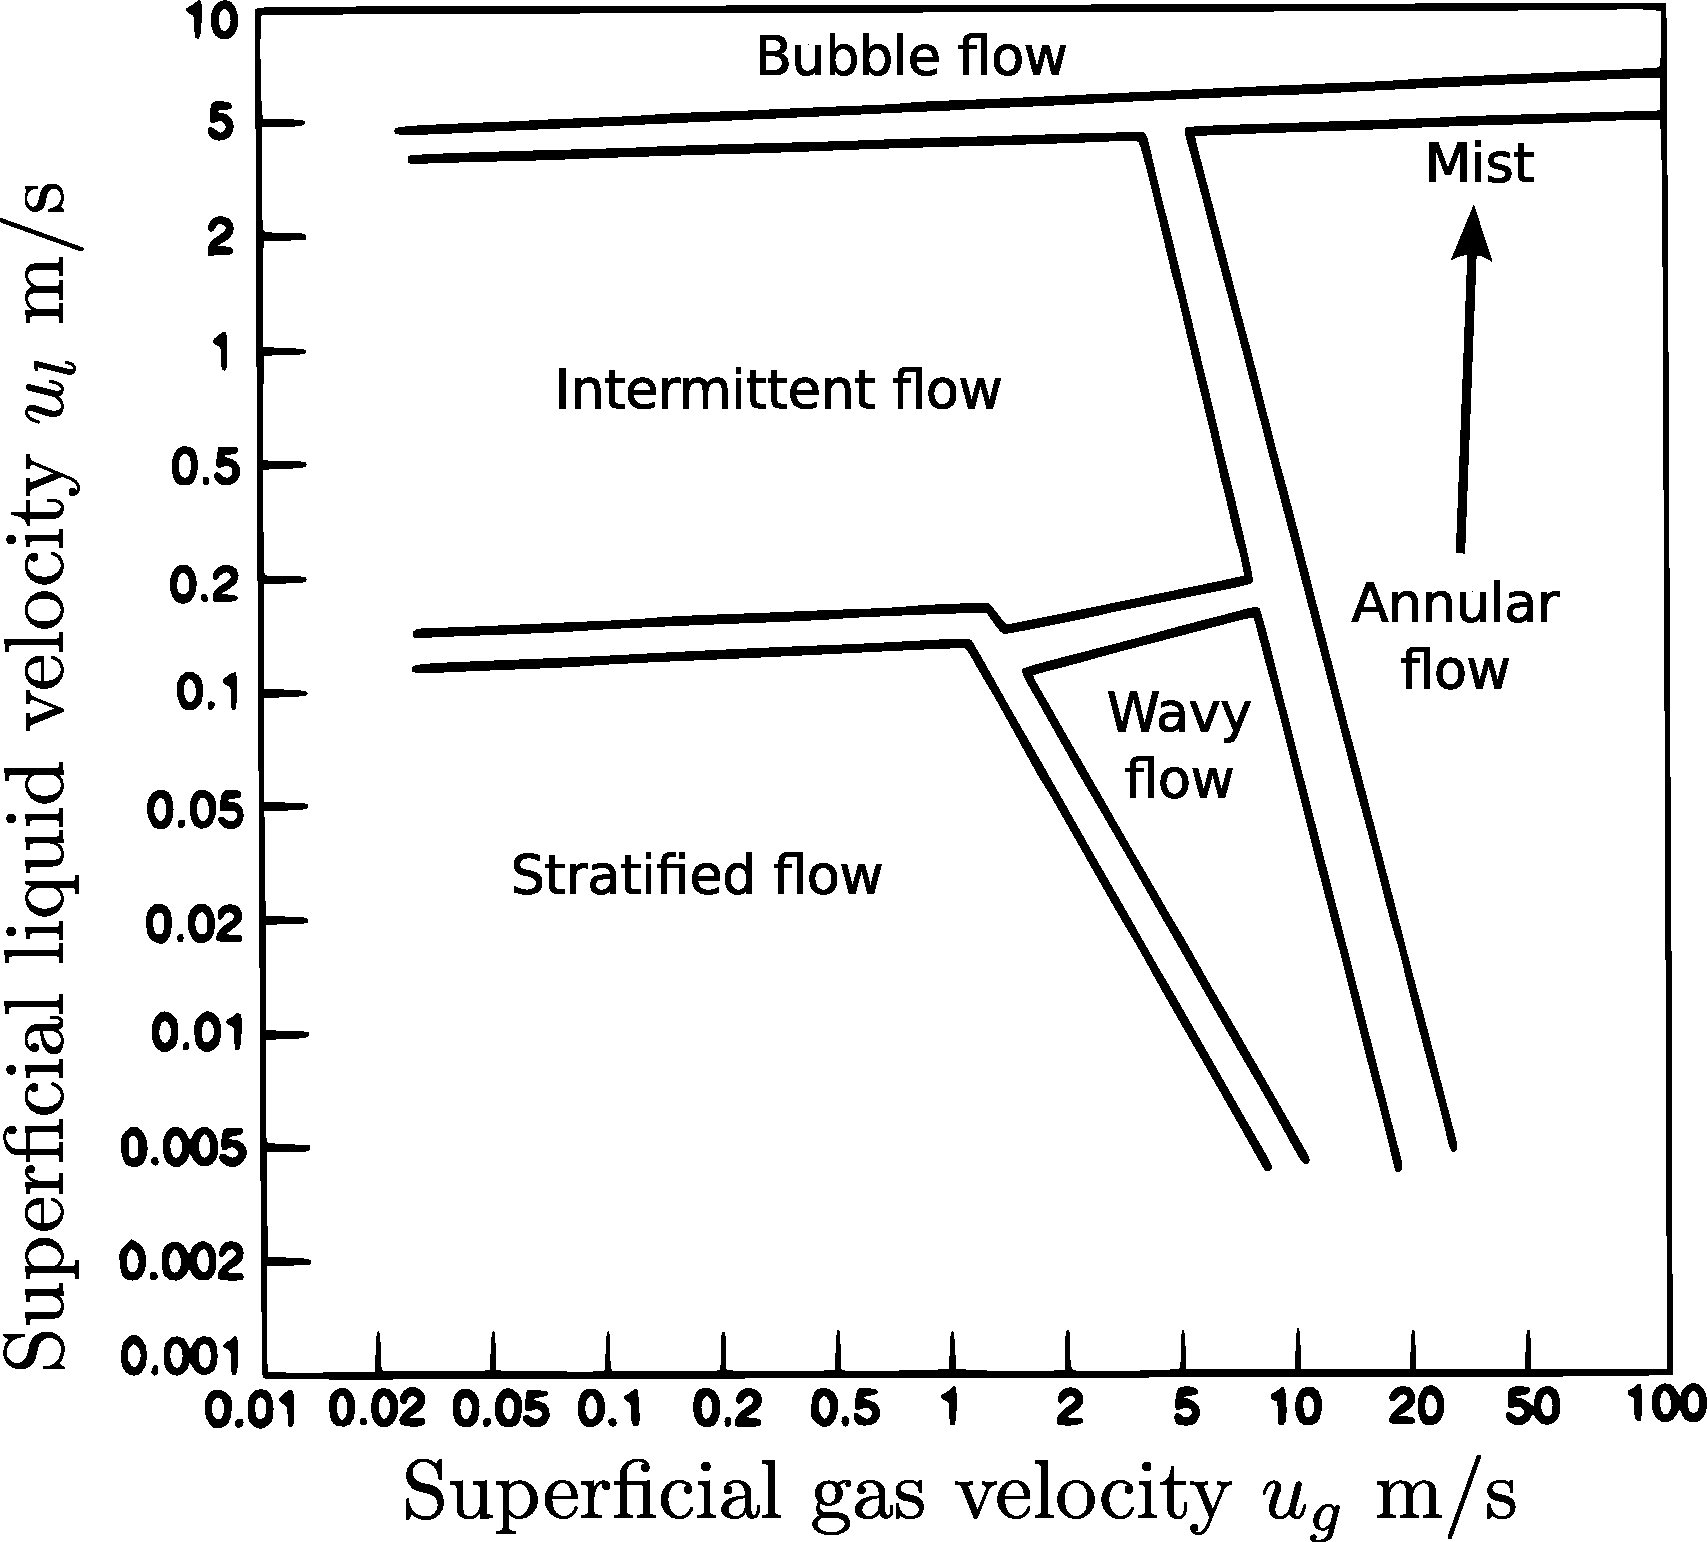
\includegraphics[width=0.6\textwidth,clip]{figures/Chhabra_richardson_flow_map}
    \end{center}
    \caption{Chhabra and Richardson flow pattern map.}
  \end{figure}

  \newpage{\bf Heat Transfer:}\\*
  Stefan-Boltzmann constant $\sigma=5.6703\times10^{-8}$~W/m${}^2$~K${}^4$
  
  Forster-Zuber pool-boiling coefficient\\*
  \begin{align*}
    h_{nb}=0.00122\frac{k_L^{0.79}\, C_{p,L}^{0.45}\, \rho_L^{0.49}}{\gamma^{0.5}\,\mu_L^{0.29}\,h_{fg}^{0.24}\,\rho_G^{0.24}}\left(T_w - T_{sat}\right)^{0.24}\left(p_w-p_{sat}\right)^{0.75}
  \end{align*}

  Mostinski correlations: ({\bf Note}, for these correlations the
  pressures are in units of bar)
  \begin{align*}
    h_{nb} = 0.104\,p_c^{0.69}\,q^{0.7}\left[1.8\left(\frac{p}{p_c}\right)^{0.17}+4\left(\frac{p}{p_c}\right)^{1.2}+10\left(\frac{p}{p_c}\right)^{10}\right]
  \end{align*}
  Mostinski critical heat flux.
  \begin{align*}
    q_c = 3.67\times10^4\,p_c\left(\frac{p}{p_c}\right)^{0.35}\left[1-\frac{p}{p_c}\right]^{0.9}
  \end{align*}

  Nusselt number
  \begin{align*}
    \text{Nu} = \frac{h\,L}{k}
  \end{align*}
  \begin{table}[ht!]
    \begin{center}
      \begin{tabular}{|p{3cm}|p{3cm}|p{3cm}|}\hline
        $\text{Ra}=\text{Gr}\,\text{Pr}$ & $C$ & $m$\\\hline
        $< 10^{4}$ & 1.36 & 1/5\\
        $10^{4}$--$10^{9}$ & 0.59 & 1/4 \\
        $>10^{9}$ & 0.13 & 1/3\\\hline
      \end{tabular}
      \caption{\label{tab:conv}Free convection coefficients for isothermal vertical
        plates in the empirical relation $\text{Nu}=C\left(\text{Gr}\,\text{Pr}\right)^m$.
        % The values are taken from Table~7-1 in ``Heat Transfer'' by J.\
        % P.\ Holman.
      }
    \end{center}
  \end{table}
  % \begin{table}[h!]
  %   \begin{center}
  %     \caption{Fourier's Law in all coordinate systems}
  %     
  %     \begin{tabular}{c|c|c}
  %       Rectangular & Cylindrical & Spherical \\
  %       \hline\noalign{\smallskip}
  %       $q_x = -k\frac{\partial T}{\partial x}$ &
  %       $q_r = -k\frac{\partial T}{\partial r}$ &
  %       $q_r = -k\frac{\partial T}{\partial r}$
  %       \\\noalign{\smallskip}%
  %       $q_y = -k\frac{\partial T}{\partial y}$
  %       & $q_\theta = -k\frac{1}{r}\frac{\partial T}{\partial \theta}$ 
  %       & $q_\theta = -k\frac{1}{r}\frac{\partial T}{\partial \theta}$ \\\noalign{\smallskip}
  %       $q_z = -k\frac{\partial T}{\partial z}$
  %       & $q_z = -k\frac{\partial T}{\partial z}$ 
  %       & $q_\phi = -k\frac{1}{r\,\sin\theta}\frac{\partial T}{\partial \phi}$
  %     \end{tabular}
  %   \end{center}
  % \end{table}

  {\bf Diffusion}\\*
  Stefan's law
  \begin{align*}
    N_{s,r} = -D \frac{c}{1-x}\frac{\partial x}{\partial r}
  \end{align*}
\end{datasheet}

\paperend
\end{document}
